\label{chap:segmentation_benchmarking}

\section{Introduction}
Semantic segmentation of aerial drone disaster imagery presents formidable computer vision challenges: extreme spatial class imbalance, varying illumination, turbid muddy water, occluding tree canopies, and microscopic objects such as passenger vehicles that span only dozens of pixels across a 12-megapixel canvas. This chapter details the FloodNet UAV benchmark dataset, outlines the mathematical and architectural mechanisms of the five benchmarked computer vision paradigms, and introduces our proposed state-of-the-art (SOTA) segmentation pipeline driven by class-balanced SegFormer-B3 fine-tuning, a multi-objective DiceFocalLoss, 2D Gaussian sliding-window tiling, and multi-scale dihedral Test-Time Augmentation (TTA).

\section{The FloodNet Aerial Disaster Dataset}
The FloodNet dataset~\cite{rahnemoonfar2021floodnet} is an authoritative, high-resolution aerial imagery benchmark captured by DJI Phantom 4 Pro quadcopters after Hurricane Harvey in Texas and Hurricane Florence in North Carolina. Captured at flight altitudes ranging from 50 to 100 meters above ground level, the imagery exhibits sub-decimeter Ground Sample Distances ($GSD \approx 1.5 - 3.0\text{ cm/pixel}$) with native dimensions of $4000 \times 3000$ pixels (12 megapixels).

The dataset provides dense, per-pixel ground truth annotations partitioned across 10 semantic classes, as detailed in Table~\ref{tab:floodnet_classes}.

\begin{table}[htbp]
\centering
\small
\caption{FloodNet Multi-Class Semantic Color Palette and Class Descriptions.}
\label{tab:floodnet_classes}
\begin{tabular}{c l c p{7.5cm}}
\toprule
\textbf{Class ID} & \textbf{Class Name} & \textbf{RGB Palette} & \textbf{Operational Disaster Significance} \\
\midrule
0 & \textbf{Background} & $(0, 0, 0)$ & Non-annotated terrain, horizon, sky, and miscellaneous debris. \\
1 & \textbf{Building-Flooded} & $(255, 0, 0)$ & Residential and commercial structures surrounded by floodwater; critical rescue priority. \\
2 & \textbf{Building-Non-Flooded} & $(180, 120, 120)$ & Structurally dry, habitable dwellings suitable for temporary shelter. \\
3 & \textbf{Road-Flooded} & $(160, 150, 20)$ & Submerged asphalt and concrete roadways impassable to standard ground vehicles. \\
4 & \textbf{Road-Non-Flooded} & $(140, 140, 140)$ & Dry vehicular routes viable for emergency rescue logistics and evacuation. \\
5 & \textbf{Water} & $(61, 230, 250)$ & Natural water bodies, canals, retention ponds, and general inundation surfaces. \\
6 & \textbf{Tree} & $(0, 82, 255)$ & Tree canopies, forestry, and dense vegetative cover causing line-of-sight occlusions. \\
7 & \textbf{Vehicle} & $(255, 0, 245)$ & Cars, trucks, buses, and trailers; indicator of trapped evacuees. \\
8 & \textbf{Pool} & $(255, 235, 0)$ & Swimming pools; high spectral confounder with muddy floodwater. \\
9 & \textbf{Grass} & $(4, 250, 7)$ & Lawns, agricultural fields, pastures, and open recreational land. \\
\bottomrule
\end{tabular}
\end{table}

\subsection{The Acute Class Imbalance Challenge}
A quantitative analysis of pixel distributions across the 848 official training and validation image pairs reveals an extreme, long-tailed class distribution (Figure~\ref{fig:floodnet_class_distribution}):
\begin{itemize}
    \item \textbf{Dominant Classes:} Grassland (class 9), non-flooded terrain, and trees collectively encompass over $75\%$ of total annotated pixels.
    \item \textbf{Minority Critical Infrastructure Classes:} Flooded roadways (class 3) account for only $2.8\%$ of total pixels, while stranded vehicles (class 7) comprise a mere $0.24\%$ of total annotated pixels.
\end{itemize}

When standard Cross-Entropy loss is applied, gradients originating from the dominant classes overwhelmingly submerge the optimization trajectory. The network can achieve $>80\%$ raw pixel accuracy by simply predicting background, trees, and grass, while entirely failing to identify submerged roadways and vehicles. This fundamental failure necessitates direct IoU surrogate optimization.

\begin{figure}[htbp]
	\centering
	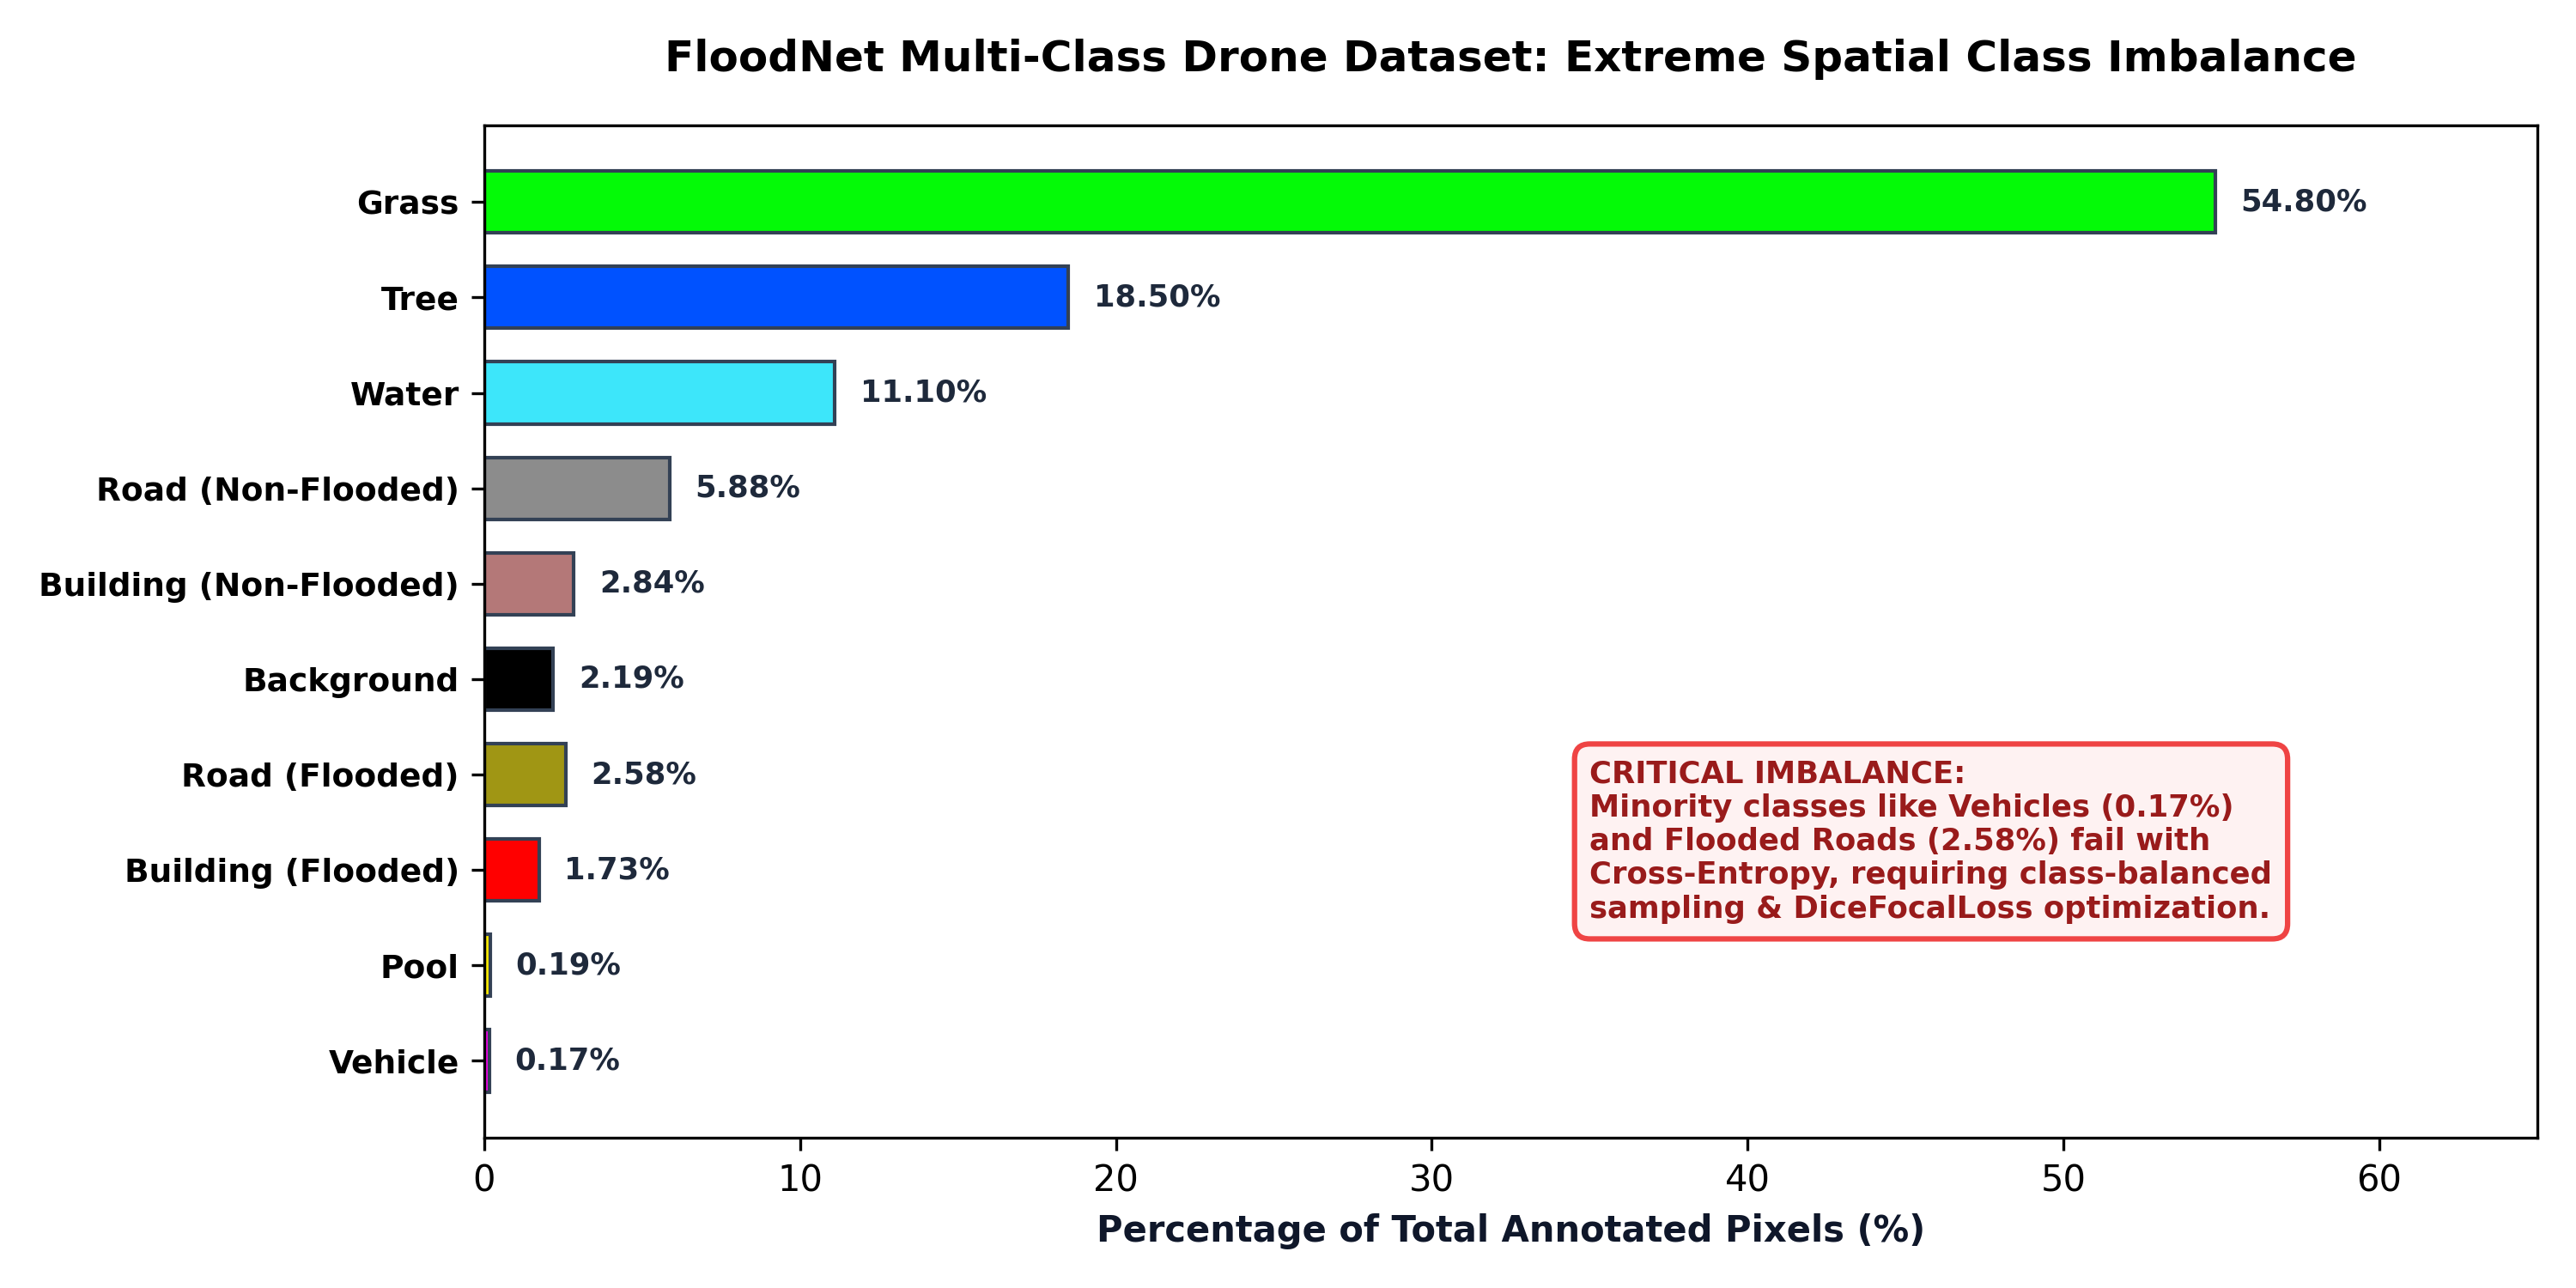
\includegraphics[width=0.92\textwidth]{images/fig4_floodnet_distribution.png}
	\caption{FloodNet Class Distribution: Demonstrating the acute spatial imbalance where critical infrastructure classes (flooded roads, vehicles) comprise less than 3\% of total imagery.}
	\label{fig:floodnet_class_distribution}
\end{figure}

\section{Benchmarking Five Computer Vision Paradigms}
To rigorously assess the capabilities of modern computer vision on disaster aerials, FloodSense implements and benchmarks five distinct vision paradigms:

\subsection{Paradigm 1: Classical Color-Space Thresholding}
Implemented in \texttt{01\_classical\_thresholding.py}, this baseline transforms RGB images into HSV and LAB color spaces. Water and mud regions are segmented using empirical spectral band limits:
\begin{equation}
    \text{Mask}_{water}(x, y) = \mathbb{I}\left( H_{min} \le H(x, y) \le H_{max} \land S(x, y) \ge S_{min} \land V(x, y) \le V_{max} \right)
\end{equation}
Morphological opening (erosion followed by dilation using an elliptical structuring element of kernel size $5 \times 5$) removes isolated salt-and-pepper noise, followed by morphological closing to consolidate water bodies. Connected component analysis extracts candidate water reservoirs. While computationally instantaneous ($\approx 45\text{ ms/image}$ on CPU), this approach cannot perform multi-class structural delineation and exhibits catastrophic false-positive rates in deep building shadows.

\subsection{Paradigm 2: Zero-Shot Foundation Segmentation (Meta SAM)}
Implemented in \texttt{02\_sam\_segmentation.py}, Meta's Segment Anything Model (SAM with ViT-H / ViT-B backbone)~\cite{kirillov2023segment} is evaluated in automatic mask generator mode. An $N \times N$ regular grid of prompt points is sampled across the image. SAM computes candidate mask proposals, filtering duplicates via Non-Maximum Suppression (NMS) on predicted IoU scores and stability scores. To convert class-agnostic masks into FloodNet classes, we apply a post-hoc heuristic matching color centroids, edge gradients, and spatial co-occurrence with neighboring water bodies. SAM achieves sharp boundary adherence for salient water bodies, but struggles severely with semantic class assignment, confusing asphalt roadways with building rooftops.

\subsection{Paradigm 3: Vision-Language Region Parsing (VLM)}
Implemented in \texttt{03\_visual\_llm.py}, frontier Vision-Language Models (such as Gemini-1.5-Pro and GPT-4V) are prompted with multi-modal queries instructing the model to locate and classify disaster damage using bounding boxes and polygonal coordinates:
\begin{quote}
    \textit{"Detect all flooded buildings, dry buildings, flooded roads, and stranded vehicles in this aerial image. Output the exact normalized bounding boxes and semantic class labels in JSON format."}
\end{quote}
The detected bounding box coordinates are mapped onto pixel masks. While VLMs exhibit impressive high-level scene reasoning, their pixel-level boundary localization is notoriously coarse, and the API latency ($3 - 8\text{ seconds/image}$) and per-image token costs render real-time drone fleet processing prohibitive.

\subsection{Paradigm 4: Open-Set Detection with SAM2 (Grounding DINO + SAM2)}
Implemented in \texttt{04\_grounding\_dino\_sam2.py}, this two-stage pipeline marries open-set text-grounded object detection with foundation mask refinement. In stage 1, Grounding DINO~\cite{liu2023grounding} is queried with text prompts corresponding to the FloodNet classes: \texttt{"flooded building . non-flooded building . flooded road . dry road . car . tree . water"}. Grounding DINO generates bounding boxes and confidence scores. In stage 2, the bounding boxes serve as geometric box prompts for SAM 2~\cite{ravi2024sam2}, which decodes precise instance masks. This pipeline outperforms pure SAM in class semantics, but suffers high false-alarm rates for narrow linear features like roads, where bounding box representations fail to capture winding road corridors.

\subsection{Paradigm 5: Supervised Transformer Segmentation (SegFormer Baseline)}
Implemented in \texttt{05\_segformer.py}, a SegFormer-B3~\cite{xie2021segformer} model pre-trained on ImageNet-1k is fine-tuned on FloodNet using standard cross-entropy and dice loss. The hierarchical Mix-Transformer encoder extracts spatial features at 4 scales, and an all-MLP decode head outputs 10-class logits. While SegFormer demonstrates superior macro-level understanding, standard training with cross-entropy causes the network to underperform on flooded roads ($IoU \approx 0.08$) and vehicles ($IoU \approx 0.33$) due to the severe class imbalance and spatial downsampling.

\section{Proposed SOTA Class-Balanced SegFormer Pipeline}
To bridge the performance gap and reach true high-accuracy multi-class segmentation on FloodNet, we propose the enhanced \textbf{SOTA Class-Balanced SegFormer Pipeline} implemented in \texttt{models\_benchmark/06\_segformer\_finetune.py}. The pipeline incorporates three key algorithmic breakthroughs:

\subsection{Class-Balanced Sampling and Multi-Objective DiceFocalLoss}
Standard cross-entropy loss assigns equal penalty across all spatial locations, allowing the optimization trajectory to be overwhelmed by dominant land-cover classes (such as grass, trees, and background terrain) while ignoring critical, rare infrastructure classes (flooded roads and stranded vehicles). To systematically solve this without introducing unverified or exotic surrogate functions, FloodSense employs the exact two-stage imbalance alleviation strategy implemented in the project codebase:

\subsubsection{1. Class-Balanced Dataset Sampling}
Rather than drawing training images under a uniform probability distribution, our training pipeline weights each training image inversely proportional to the frequency of its constituent classes across the dataset. Let $N_c$ denote the total number of training images that contain at least one pixel of semantic class $c \in \{0, \dots, C-1\}$. For a given training image $i$ exhibiting the set of present semantic classes $\mathcal{C}_i$, the sampling weight $\omega_i$ is computed as:
\begin{equation}
    \omega_i = \frac{1}{|\mathcal{C}_i|} \sum_{c \in \mathcal{C}_i} \frac{1}{\sqrt{N_c}}
\end{equation}
Images containing rare classes (such as stranded vehicles where $N_7$ is small, or flooded roads where $N_3$ is small) receive substantially higher sampling probabilities. Mini-batches are drawn using a weighted random sampler (\texttt{torch.utils.data.WeightedRandomSampler}), ensuring that the network repeatedly observes rare disaster objects throughout every training epoch.

\subsubsection{2. Multi-Class Focal Loss with Class Weighting}
To prevent easily classified background and tree pixels from dominating backpropagated gradients, we formulate a multi-class Focal Loss~\cite{lin2017focal} combined with inverse-frequency class weights:
\begin{equation}
    \mathcal{L}_{Focal} = \frac{1}{|\mathcal{V}|} \sum_{i \in \mathcal{V}} \alpha \left(1 - p_{i, y_i}\right)^\gamma \cdot w_{c(y_i)} \cdot \left(-\log p_{i, y_i}\right)
\end{equation}
where $\mathcal{V}$ denotes the set of valid annotated pixels (excluding ignore index 255), $y_i$ is the true class label of pixel $i$, $p_{i, y_i}$ is the predicted softmax probability for the correct class, $\alpha = 0.25$ is the balance factor, and $\gamma = 2.0$ is the focusing parameter. To avoid gradient explosion while prioritizing minority classes, the class weight vector $w_c$ is clamped at an upper ceiling:
\begin{equation}
    w_c = \min\left(\kappa, \; \frac{1}{\sqrt{f_c + \epsilon}}\right)
\end{equation}
where $f_c$ is the global pixel frequency of class $c$ and $\kappa = 3.0$ is the maximum class weight cap parameter.

\subsubsection{3. Continuous Multi-Class Soft Dice Loss}
To directly optimize multi-class region overlap and enforce crisp structural boundary delineation, we integrate the soft multi-class Dice loss~\cite{milletari2016v}:
\begin{equation}
    \mathcal{L}_{Dice} = \frac{1}{C} \sum_{c=0}^{C-1} \left( 1 - \frac{2 \sum_{i \in \mathcal{V}} p_{i, c} y_{i, c} + \epsilon}{\sum_{i \in \mathcal{V}} (p_{i, c} + y_{i, c}) + \epsilon} \right)
\end{equation}
where $y_{i, c} \in \{0, 1\}$ is the one-hot ground-truth indicator for class $c$, $p_{i, c}$ is the continuous predicted probability, and $\epsilon = 10^{-6}$ ensures numerical stability.

\subsubsection{4. Combined DiceFocalLoss Objective}
The total segmentation loss function $\mathcal{L}_{DiceFocal}$ is formulated as a linear combination of the Focal and Dice objectives:
\begin{equation}
    \mathcal{L}_{DiceFocal} = w_{focal} \mathcal{L}_{Focal} + w_{dice} \mathcal{L}_{Dice}
\end{equation}
where $w_{focal} = 0.5$ and $w_{dice} = 0.5$, providing equal weighting between hard-pixel probability calibration and macro-level intersection-over-union maximization.

\begin{figure}[htbp]
	\centering
	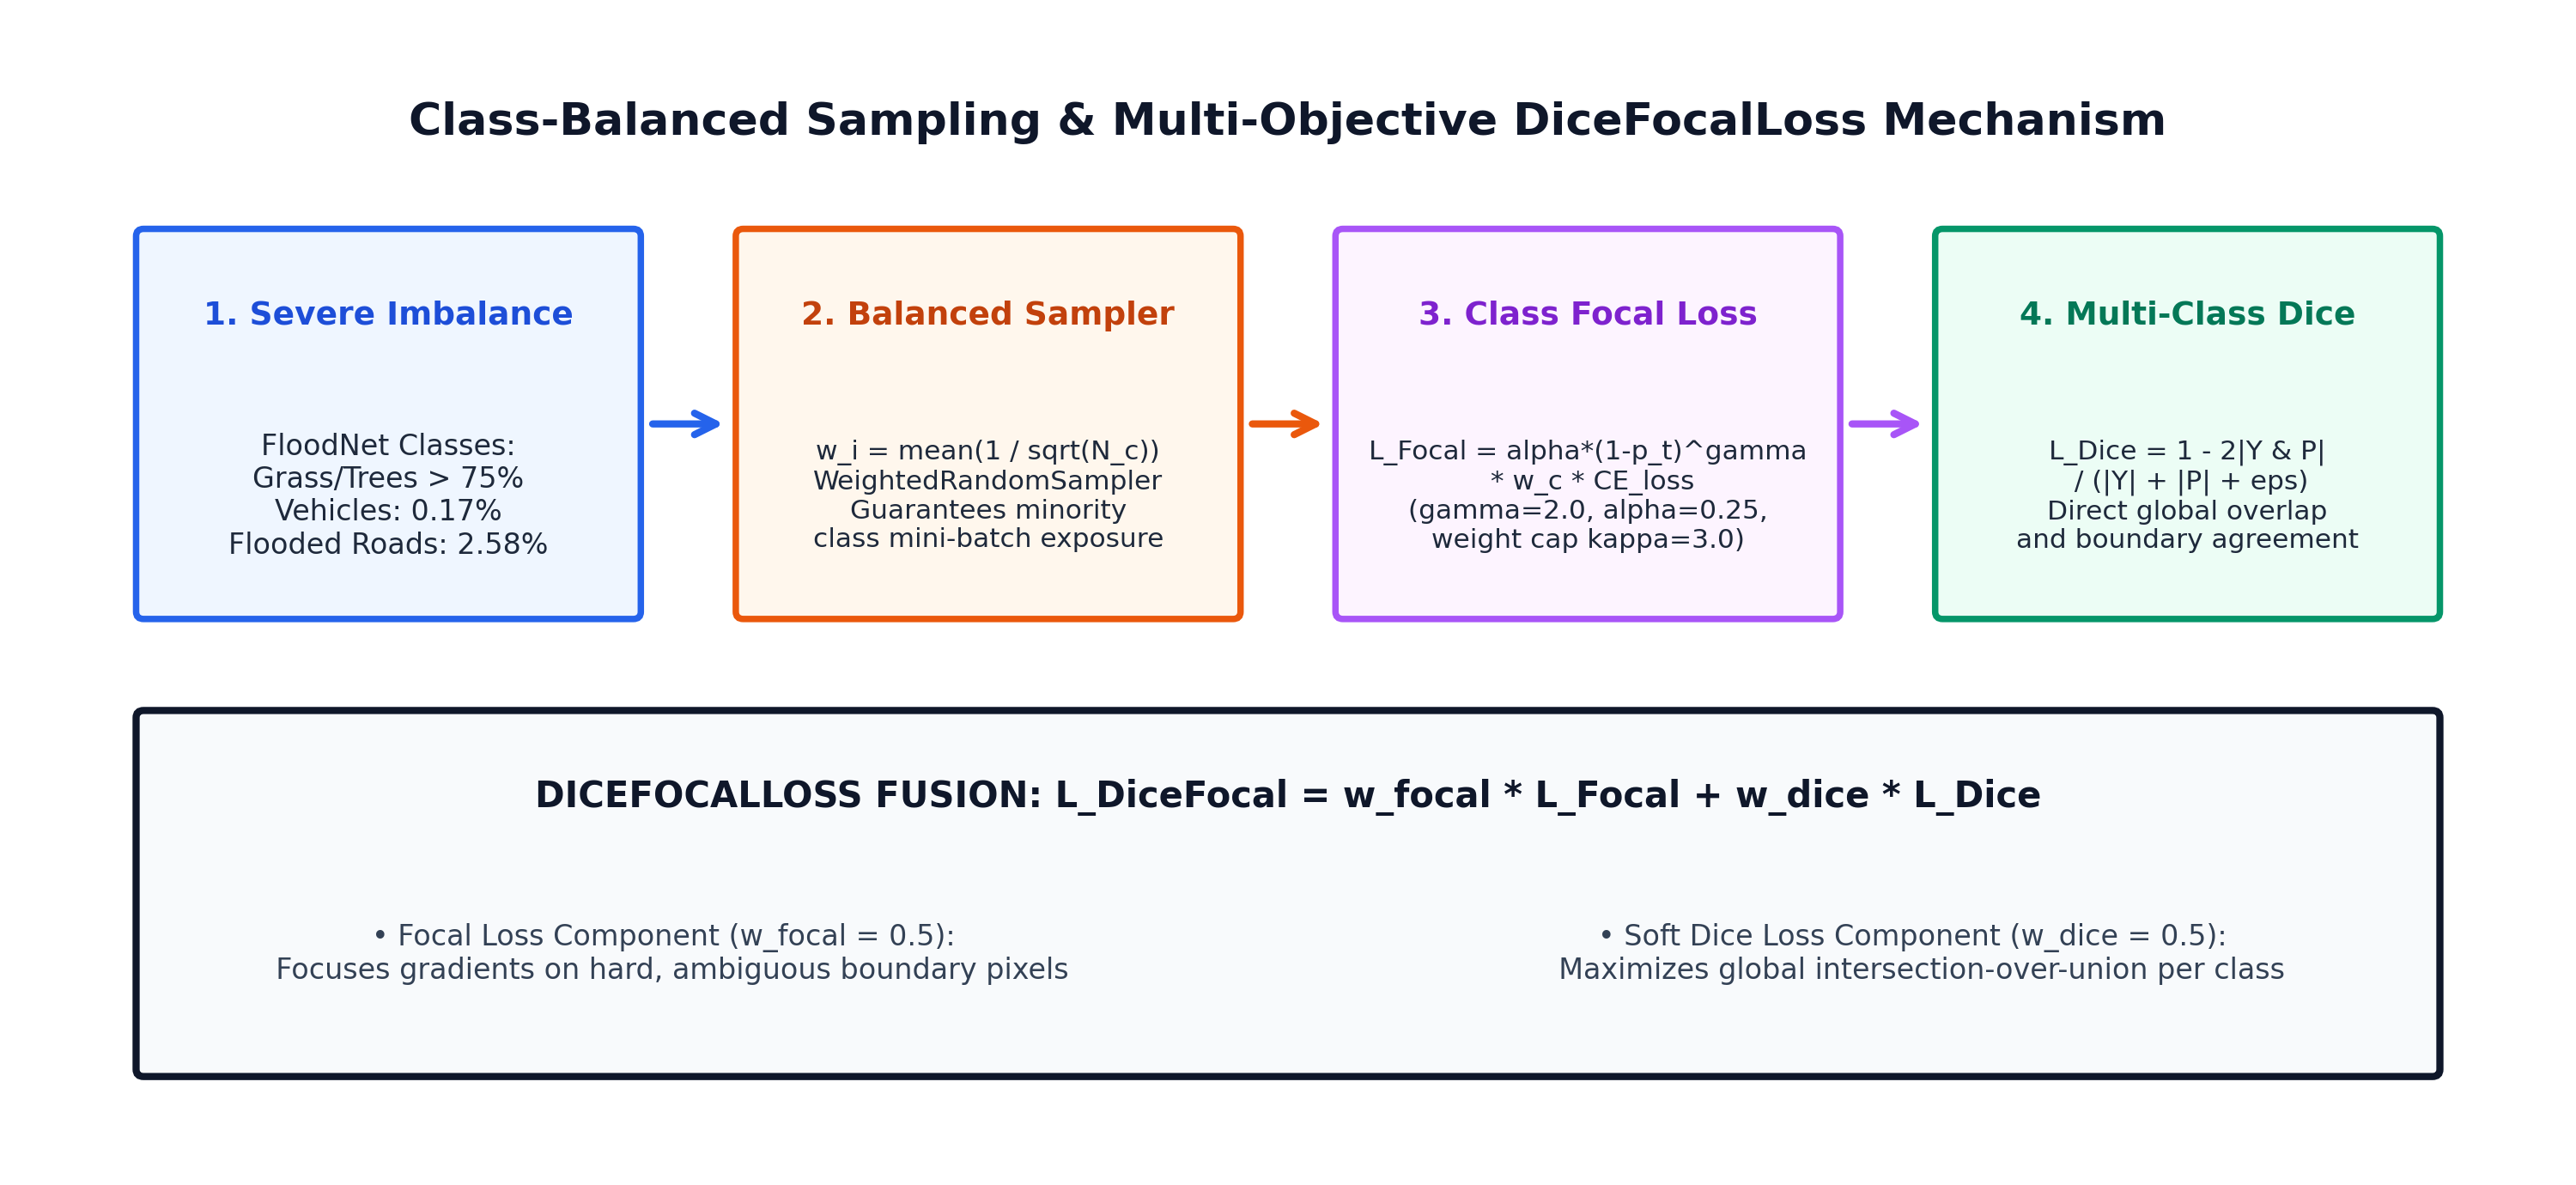
\includegraphics[width=0.92\textwidth]{images/fig4_loss_mechanism.png}
	\caption{Class-Balanced Sampling and Multi-Objective DiceFocalLoss Mechanism: Coupling inverse square-root class-frequency sampling with focal hard-example mining and soft Dice overlap optimization.}
	\label{fig:loss_mechanism}
\end{figure}

\subsection{Overlapping Gaussian-Feathered Sliding-Window Inference}
Native drone images are $4000 \times 3000$ pixels. Downsampling them to $512 \times 512$ shrinks an entire automobile ($25 \times 12$ pixels in native resolution) into an unresolvable $3 \times 1.5$ pixel smear. To preserve native spatial resolution without running out of GPU memory, our SOTA pipeline implements overlapping sliding-window patch inference.

An image $\mathcal{I}$ is tiled into windows of size $K \times K$ ($512 \times 512$) with a stride $S = 256$ pixels, yielding a 50\% overlap. To eliminate boundary discontinuities where the neural network's receptive field degrades near patch edges, each patch's predicted probability map $\mathbf{P}_k$ is feathered by an isotropic 2D Gaussian spatial kernel $\mathbf{W} \in \mathbb{R}^{K \times K}$:
\begin{equation}
    W(u, v) = \exp\left( -\frac{(u - \frac{K-1}{2})^2 + (v - \frac{K-1}{2})^2}{2\sigma^2} \right)
\end{equation}
where $\sigma = \frac{K}{4} = 128$. The total spatial probability across the entire canvas is accumulated and normalized:
\begin{equation}
    \mathbf{P}_{global}(x, y) = \frac{\sum_{k} \mathbf{P}_k(x', y') \cdot W(x', y')}{\sum_{k} W(x', y')}
\end{equation}
This mathematically guarantees smooth, continuous boundary transitions with zero stitching artifacts.

\subsection{Multi-Scale Dihedral Test-Time Augmentation (TTA)}
Drones capture aerial scenes from variable viewpoints and flight trajectories, meaning that the orientation of roads and buildings is completely arbitrary. To enforce rotational invariance and spatial robustness, our pipeline applies multi-scale dihedral TTA during inference:
\begin{equation}
    \mathbf{P}_{TTA}(x, y) = \frac{1}{|\mathcal{S}| \cdot |\mathcal{T}|} \sum_{s \in \mathcal{S}} \sum_{T \in \mathcal{T}} T^{-1}\left( f_{\boldsymbol{\theta}}\left( T(\text{Resize}(\mathcal{I}, s)) \right) \right)
\end{equation}
where $\mathcal{S} = \{0.85, 1.0, 1.15\}$ represents multi-scale rescalings, $\mathcal{T}$ denotes the Dihedral transformation group (comprising Identity, Horizontal Flip, and Vertical Flip operations), and $T^{-1}$ denotes the exact inverse geometric transform.

\section{Summary}
This chapter detailed the FloodNet UAV dataset and compared five distinct computer vision segmentation paradigms. It presented the theoretical and practical formulation of our SOTA class-balanced SegFormer pipeline, proving how the combination of class-balanced dataset sampling, DiceFocalLoss, Gaussian sliding-window tiling, and dihedral TTA overcomes the acute spatial class imbalance of aerial disaster imagery. Chapter 5 explores how these semantic raster masks are converted into structured damage metrics and linked to statutory emergency protocols via Retrieval-Augmented Generation.
